\section{Analysis}

\subsection{Reaching equilibrium}
The system was considered to be in equilibrium after a pre-simulation over 50.000 timesteps. As can be seen in figure \ref{findeq}, 50.000 timesteps is way more than enough for the energies to be in equilibrium. After just a few thousand steps they fluctruate only a little around a constant average value. For the MSD and Debye temperature, it is harder to say directly from the plot wether the system has reached equilibrium or not.
\begin{figure}[H]
	\centering
	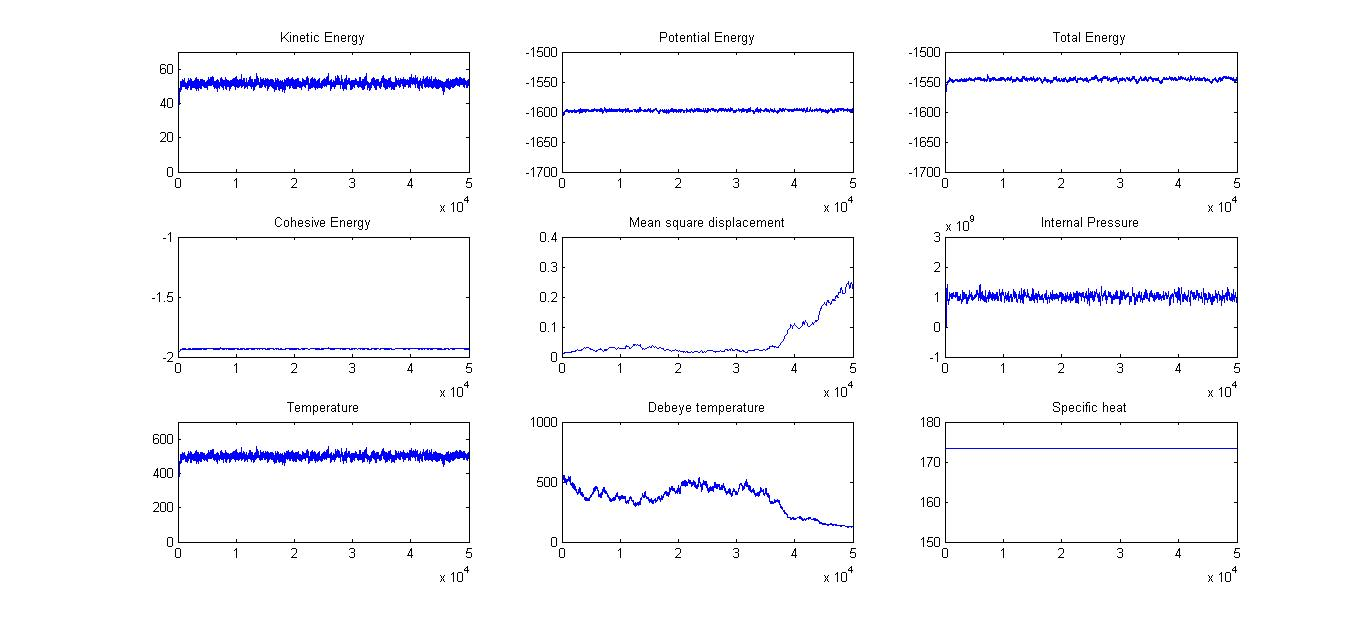
\includegraphics[width=0.7\textwidth]{findEqSurface.jpg}
	\caption{Plots of the different properties during the "pre equilibrium" surface simulation.}
	\label{findeq}
\end{figure}
\subsection{Total and cohesive energy}
Theoretically, the total energy should be constant during the whole simulation (energy conservation). However, we can se som minor fluctruations of the value, at most 0.01 \% of the average value (See fig. \ref{totale} (it behaves the same in both bulk and surface simulations). This is most probably depending on that rounded values have to be used in the calculations. Since the fluctruations are so small after reaching equilibrium, we consider it being constant enough to run a descent simulation. 
The value of the total energy equals to the sum of the potantial and the kinetic energy, just like it should theoretically.
\subsubsection{Cohesive energy}
The cohesive energy has an average value of 1.93 eV in the main test simulation. It is hard to find any tabulated values to compare with for that temperature, so we made a test run at T=0K also. Here, the average cohesive energy was 2.34 eV, which is not the same but within a reasonable range from the tabulated value wich was found to be 2.95 eV \cite{kittel}.

\subsection{Kinetic energy and temperature}
The kinetic energy and temperature are strictly connected to eachother. The Andersen thermostat keeps the temperature close to its starting value during the whole simulation.

\subsection{Potential energy}
After reaching equilibrium, the potential energy fluctruates with less than 0.1\%. The fluctruations ar directly related to the fluctruations of the kinetic energy, together they sum up to the total energy.

\subsection{MSD and diffusion coefficient}
The mean square displacement (MSD) shows how much the atoms have moved in average from their original position. This divided by 6*the-total-time Results in the diffusion coefficient which can be used to see that equilibrium is reached. The graph in figure \ref{fig:Diffusion_coeff} shows how the diffusion coefficient drops over time. The run is made from start ant for 50,000 timesteps and shows that the bulk reaches equilibrium. 
\begin{figure}[ht]
	\centering
	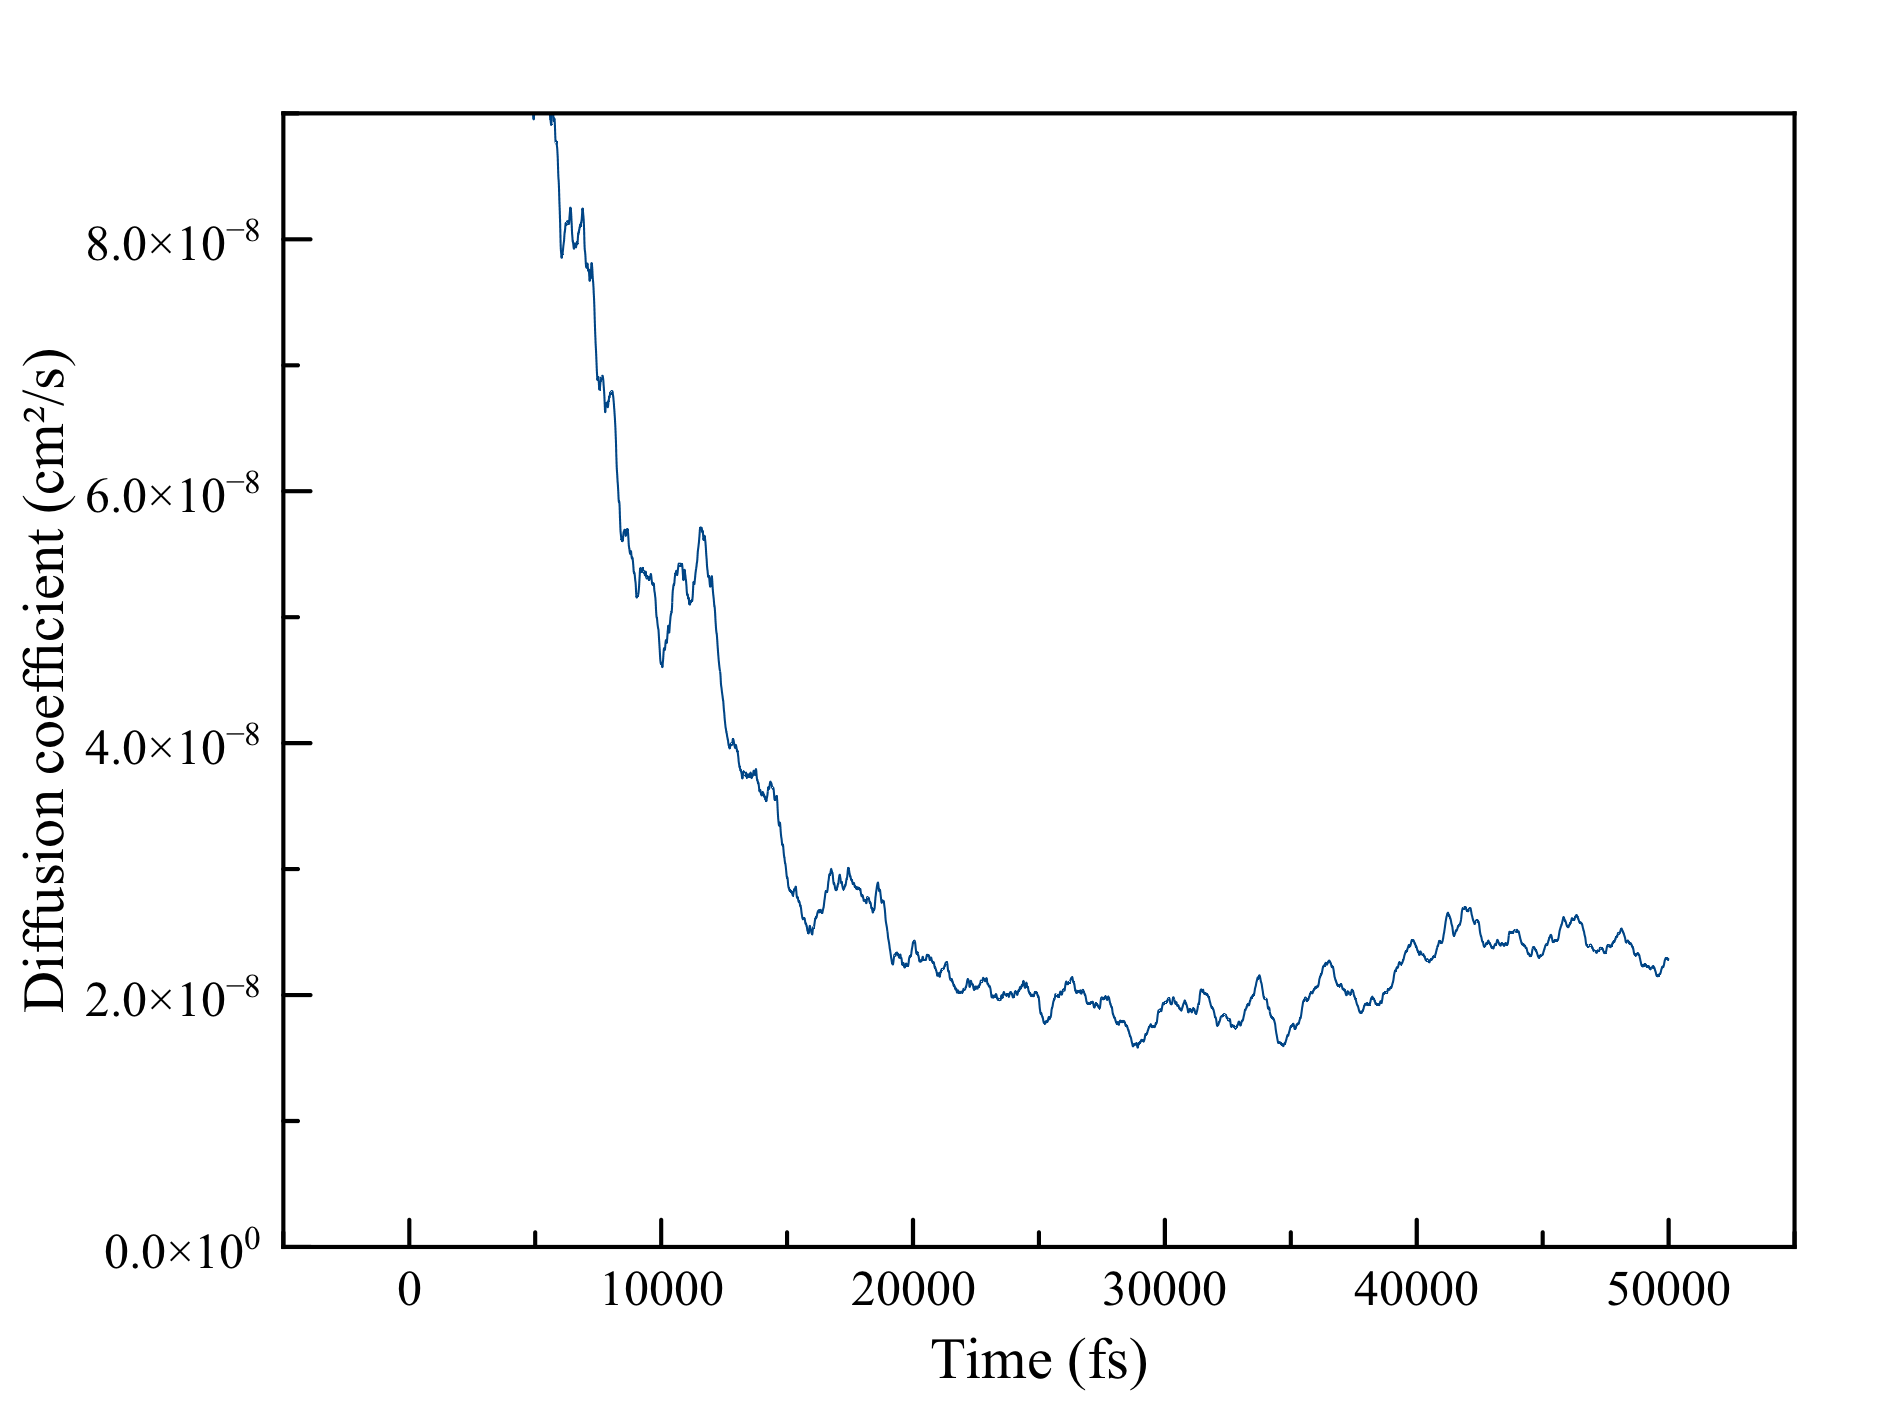
\includegraphics[width=0.8\textwidth]{Diffusion_coeff.png}
	\caption{Diffusion coefficient over time}
	\label{fig:Diffusion_coeff}
\end{figure}
Furthermore can be seen in figure \ref{fig:diffusion_coeff_surface}, which is a graph of diffusion coefficient for a surface ran from equilibrium, and it is at this point very stable.
\begin{figure}[ht]
	\centering
	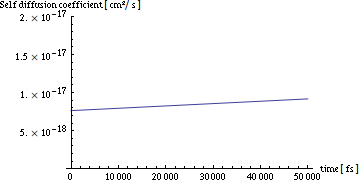
\includegraphics[width=0.8\textwidth]{diffusion_coeff_surface.png}
	\caption{Diffusion coefficient for a surface over time}
	\label{fig:diffusion_coeff_surface}
\end{figure}

\subsection{Debye temperature}
In this program the calculation of the Debye temperature is done with inverse proportion to the MSD and proportional to the temperature. The value stabilizes around 250 (see figure \ref{fig:debyetemp}) which corresponds fairly well to the tabulated properties (215K) \cite{bib:DebyeSilver}.
\begin{figure}[ht]
	\centering
	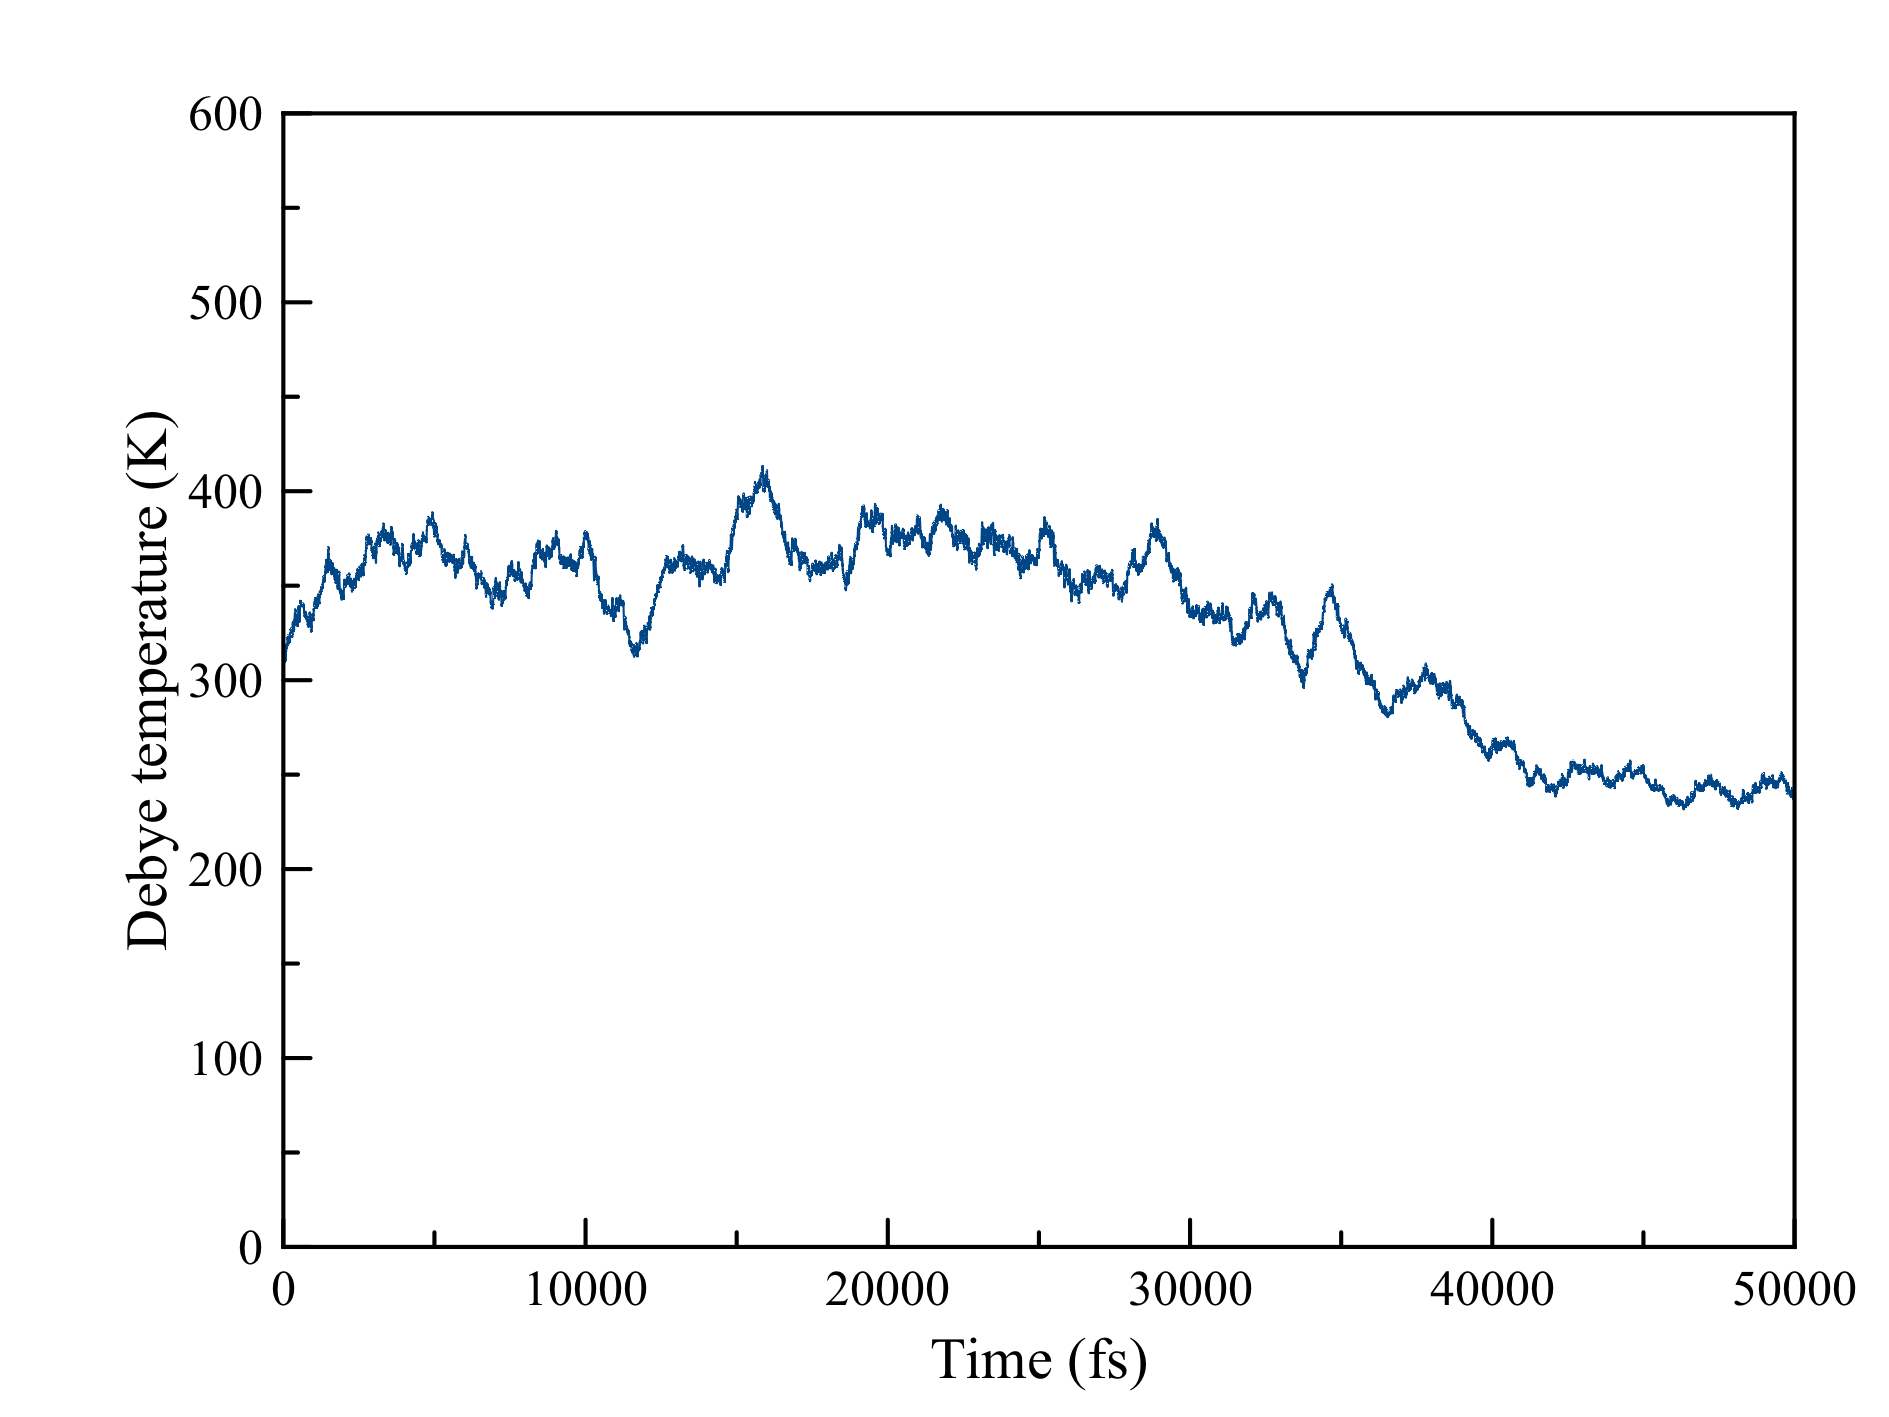
\includegraphics[width=0.8\textwidth]{debyetemp.png}
	\caption{Debye temperature for a bulk}
	\label{fig:debyetemp}
\end{figure}
For the surface simulation, the Debye Temperature will be a bit lower than for the bulk as seen in figure \ref{fig:debye_surface}.
\begin{figure}[ht]
	\centering
	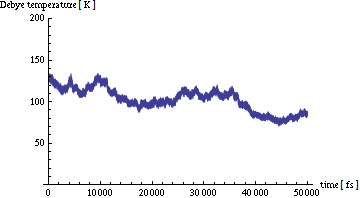
\includegraphics[width=0.8\textwidth]{debye_surface.png}
	\caption{Debye temperature for a surface}
	\label{fig:debye_surface}
\end{figure}

